\documentclass[letterpaper,10pt]{article}
\usepackage[top=2cm, bottom=1.5cm, left=1cm, right=1cm]{geometry}
\usepackage{amsmath, amssymb, amsthm,graphicx}
\usepackage{fancyhdr}
\pagestyle{fancy}

\lhead{\today}
\chead{Regression Assignment 6a}
\rhead{Justin Hood}

\newcommand{\Z}{\mathbb{Z}}
\newcommand{\Q}{\mathbb{Q}}
\newcommand{\R}{\mathbb{R}}
\newcommand{\C}{\mathbb{C}}
\newtheorem{lem}{Lemma}

\begin{document}
We shall fit a regression of the form,
\[y_t=\beta_0+\beta_1 t+\beta_2 Q_2+\beta_3 Q_3+\beta_4 Q_4+\epsilon_t\]
With $Q_i$ dummy variables for the $i^{th}$ quarter of a given year.
\begin{enumerate}
\item First, we define the dummy variables as follows.
\begin{align*}
Q_2 &= \begin{cases}
1 & t\in\text{Quarter 2}\\
0 & t\not\in\text{Quarter 2}
\end{cases}\\
Q_3 &= \begin{cases}
1 & t\in\text{Quarter 3}\\
0 & t\not\in\text{Quarter 3}
\end{cases}\\
Q_4 &= \begin{cases}
1 & t\in\text{Quarter 4}\\
0 & t\not\in\text{Quarter 4}
\end{cases}
\end{align*}
\item Next, we plot the data to analyze the overall data trends to see if we need to scale for constant seasonal variation.
\begin{center}
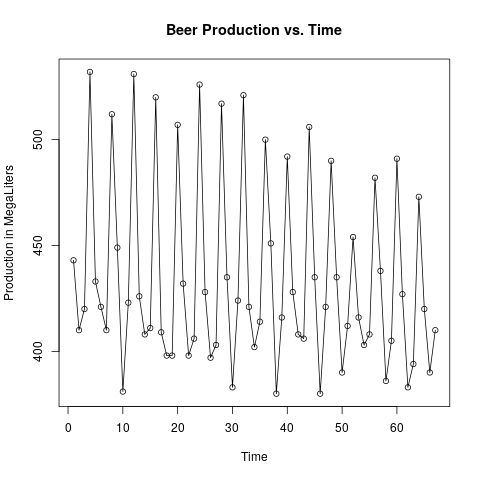
\includegraphics[scale=.8]{unlogged.png}
\end{center}
We see here that the overall trend of the data is negative, but there is no major increase or decrease in seasonal variation over the experimental region. As such, we expext $\beta_1$ to have a negative value, and we will not log or scale the $y$ variable at all to approximate constant variation.
\item What are the values of beer production for 2009? We consider the following points,
\begin{center}
\begin{tabular}{|c|c|}
\hline
Point & Definition \\\hline
$\hat{y}_{68}$ & $Q_4$ of 2008\\
$\hat{y}_{69}$ & $Q_1$ of 2009\\
$\hat{y}_{70}$ & $Q_2$ of 2009\\
$\hat{y}_{71}$ & $Q_3$ of 2009\\
$\hat{y}_{72}$ & $Q_4$ of 2009\\\hline
\end{tabular}
\end{center}
\item We now construct our prediction equation as,
\[\hat{y}=442.62153-0.35486t-35.40985Q_2-19.58440Q_3+72.78868Q_4\]
With $Q_i$ defined as above. We consider the fit as follows,
\begin{center}
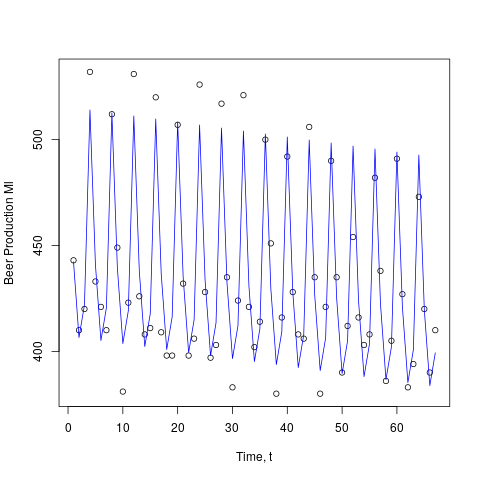
\includegraphics[scale=0.8]{Fitted.png}
\end{center}
We see that this fit fairly accurately follows the trend, and so, we may compute,
\begin{align*}
\hat{y}_{68} &= 442.62153-0.35486(68)+72.78868(1)\\
&= 491.31\text{Ml}\\
\hat{y}_{69} &= 442.62153-.035486(69)\\
&= 418.17\text{Ml}
\end{align*}
\item We now construct our prediction equation and approximate,
\begin{center}
\begin{tabular}{|c|c|c|}
\hline
$y_*$ & Prediction & Interval \\\hline
$y_{69}$ & $418.17$ & $(391.89,\ 444.44)$\\
$y_{70}$ & $382.40$ & $(356.13,\ 408.68)$\\
$y_{71}$ & $397.87$ & $(371.60,\ 424.15)$\\
$y_{72}$ & $489.89$ & $(463.50,\ 516.28)$\\\hline
\end{tabular}
\end{center}
\end{enumerate}
\end{document}
